%%%%%%%%%%%%%%%%%%%%%%%%%%%%%%%%%%%%%%%%%
% Beamer Presentation
% LaTeX Template
% Version 1.0 (10/11/12)
%
% This template has been downloaded from:
% http://www.LaTeXTemplates.com
%
% License:
% CC BY-NC-SA 3.0 (http://creativecommons.org/licenses/by-nc-sa/3.0/)
%
%%%%%%%%%%%%%%%%%%%%%%%%%%%%%%%%%%%%%%%%%

%----------------------------------------------------------------------------------------
%	PACKAGES AND THEMES
%----------------------------------------------------------------------------------------

\documentclass[10pt]{beamer}

\mode<presentation> {

% The Beamer class comes with a number of default slide themes
% which change the colors and layouts of slides. Below this is a list
% of all the themes, uncomment each in turn to see what they look like.

%\usetheme{default}
%\usetheme{AnnArbor}
%\usetheme{Antibes}
%\usetheme{Bergen}
%\usetheme{Berkeley} % Neat Contents on left
%\usetheme{Berlin}
%\usetheme{Boadilla}
%\usetheme{CambridgeUS} % Neat but breadcrumbs at top
%\usetheme{Copenhagen}
%\usetheme{Darmstadt}
%\usetheme{Dresden}
%\usetheme{Frankfurt}
%\usetheme{Goettingen} %Neat contents on right
%\usetheme{Hannover} %Neat contents on left
%\usetheme{Ilmenau}
%\usetheme{JuanLesPins}
%\usetheme{Luebeck}
%\usetheme{Madrid}
%\usetheme{Malmoe}
%\usetheme{Marburg} % Contents on right in contrast color
%\usetheme{Montpellier}
\usetheme{PaloAlto} % Contents on left
%\usetheme{Pittsburgh}
%\usetheme{Rochester}
%\usetheme{Singapore}
%\usetheme{Szeged}
%\usetheme{Warsaw}

% As well as themes, the Beamer class has a number of color themes
% for any slide theme. Uncomment each of these in turn to see how it
% changes the colors of your current slide theme.

%\usecolortheme{albatross}
%\usecolortheme{beaver}
%\usecolortheme{beetle}
%\usecolortheme{crane}
%\usecolortheme{dolphin}
%\usecolortheme{dove}
%\usecolortheme{fly}
%\usecolortheme{lily}
%\usecolortheme{orchid}
%\usecolortheme{rose}
\usecolortheme{seagull}
%\usecolortheme{seahorse}
%\usecolortheme{whale}
%\usecolortheme{wolverine}

%\setbeamertemplate{footline} % To remove the footer line in all slides uncomment this line
%\setbeamertemplate{footline}[page number] % To replace the footer line in all slides with a simple slide count uncomment this line

%\setbeamertemplate{navigation symbols}{} % To remove the navigation symbols from the bottom of all slides uncomment this line
}

\usepackage{graphicx} % Allows including images
\usepackage{booktabs} % Allows the use of \toprule, \midrule and \bottomrule in tables

%----------------------------------------------------------------------------------------
%	TITLE PAGE
%----------------------------------------------------------------------------------------

\title[Improving Outcomes in Pancreatic Surgery]{An investigation of the clinical utility of preoperative cardiopulmonary exercise testing in patients undergoing major pancreatic surgery.} % The short title appears at the bottom of every slide, the full title is only on the title page

\author{Vishnu V Chandrabalan} % Your name
\institute[UoG] % Your institution as it will appear on the bottom of every slide, may be shorthand to save space
{
University of Glasgow \\ % Your institution for the title page
\medskip
% \textit{john@smith.com} % Your email address
}
\date{\today} % Date, can be changed to a custom date

\begin{document}

\begin{frame}
\titlepage % Print the title page as the first slide
\end{frame}

\begin{frame}
\frametitle{Overview} % Table of contents slide, comment this block out to remove it
\tableofcontents % Throughout your presentation, if you choose to use \section{} and \subsection{} commands, these will automatically be printed on this slide as an overview of your presentation
\end{frame}

%----------------------------------------------------------------------------------------
%	PRESENTATION SLIDES
%----------------------------------------------------------------------------------------

%------------------------------------------------
\section{Introduction}
\subsection{Pancreatic cancer}
\begin{frame}
	\frametitle{Pancreatic cancer} %Epidemiology/outcomes
	\begin{block}{The Problem}
		\begin{itemize}
			\item 10th common but 5th common cause of cancer death
			\item Survival	1-yr: 20.8\%, 5-yr: 3.3\%, 10yr: 1.1\%
			\item Operable disease : approx 15\%
		\end{itemize}
	\end{block}
	\begin{block}{Treatment}
		\begin{itemize}
			\item Surgery + adjuvant chemotherapy only chance of cure
		\end{itemize}
	\end{block}
	\begin{block}{Pancreaticoduodenectomy}
		\begin{itemize}
			\item Complex surgery with 50\% morbidity
			\item Performed only in specialist centres
			\item Patient fitness is as important as tumour factors
		\end{itemize}
	\end{block}
\end{frame}

\begin{frame}
	\frametitle{Pancreaticoduodenectomy}
	\begin{columns}[t]
		\column{0.45\textwidth}
		\begin{figure}
			\centering
			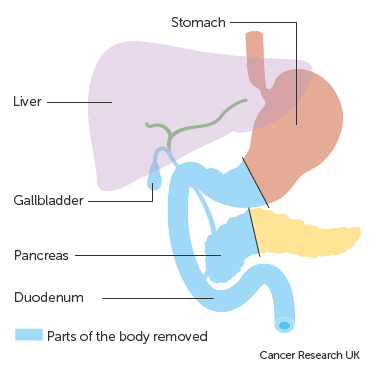
\includegraphics[width=0.8\linewidth]{whipple_schematic_pre}
			\label{fig:whipple_schematic_pre}
		\end{figure}
		{\scriptsize
			\textbf{Structures removed:}
			\begin{itemize}
			\item Head of pancreas
			\item Distal stomach, duodenum, proximal jejunum
			\item  Common bile duct, gallbladder
			\item Lymphadenectomy
			\item Venous resection in some
		\end{itemize}}
	
		
		\column{0.45\textwidth}
		\begin{figure}
			\centering
			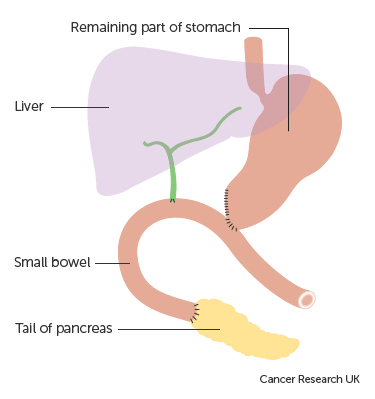
\includegraphics[width=0.8\linewidth]{whipple_schematic_post}
			\label{fig:whipple_schematic_post}
		\end{figure}
		{\scriptsize
		\textbf{Reconstruction:}
		\begin{itemize}
			\item Pancreaticojejunostomy (25\% leak rate)
			\item Hepaticojejunostomy
			\item Gastrojejunostomy
		\end{itemize}
		}
	\end{columns}
\end{frame}

\begin{frame}
	\frametitle{Complications of Surgery}
	\framesubtitle{Section 1.2.4 Pages 8-11}
	\begin{itemize}
		\item Significant improvements in mortality ($<$5\% from $>$40\%)
		\item Morbidity remains high at over 40\%
		\item Postoperative pancreatic fistula (POPF) is serious
		\item POPF can lead to other complications: Sepsis, PPH, DGE
		\item International Study Group for Pancreatic Surgery
		\item Clavien-Dindo classification of complications
	\end{itemize}
\end{frame}

\begin{frame}
	\frametitle{Adjuvant therapy}
	\framesubtitle{Section 1.3 Pages 11,13 }
	\begin{itemize}
		\item Adjuvant therapy improves survival
		\item Currently standard of care and subject of multiple trials
		\item 25\% - 50\% of patients do not receive adjuvant treatment
		\item Multiple factors including:
		\begin{itemize}
			\item Comorbidity
			\item Complications of surgery
			\item Favourable pathological features
		\end{itemize}
	\end{itemize}
\end{frame}

\subsection{CPET}
\begin{frame}
	\frametitle{Risk Stratification }
	\framesubtitle{Section 1.4 Pages 13-18 }
	\begin{itemize}
		\item Patient fitness is important determinant of outcome
		\item Effect of comorbidity on function is difficult to assess
		\item POSSUM, APACHE, mGPS, E-PASS, etc.
		\item Static measures do not predict performance under stress
		\item Do not provide targets for prehabilitation
		\item Pancreas specific risk factors of POPF
		\begin{itemize}
			\item Soft pancreas
			\item Narrow pancreatic duct
			\item Pathology not obstructing PD
			\item These factors are not modifiable
			\item Coronary artery disease! (Lin 2004)
		\end{itemize}
	\end{itemize}
\end{frame}

\begin{frame}
	\frametitle{What is CPET?}
	\framesubtitle{Section 1.5 Page 18}
	\begin{itemize}
		\item Objective measure of cardiopulmonary response to exercise
		\item Dynamic test measuring numerous parameters
		\item Cardiac, respiratory, vascular and mitochondrial function
		\item First described for preoperative assessment by Older and co-workers
		\item Widely used in general, oesophago-gastric, vascular and thoracic surgery
	\end{itemize}
\end{frame}

\begin{frame}
	\frametitle{CPET Methodology}
	\framesubtitle{Section 1.5.2 Page 20 }
	\begin{itemize}
		\item Dynamic exercise test
		\item Cycle ergometer with electronic braking and incremental workload
		\item Breath-by-breath gas analysis using a tight-fitting face mask
		\item Continuous monitoring of 12-lead ECG
		\item Initial 3-minute rest period on bike for baseline parameters
		\item Incremental work-load test to volitional fatigue
		%include picture here
	\end{itemize}
\end{frame}

\begin{frame}
	\frametitle{Physiological basis of CPET} 
	\begin{figure}
		\centering
		\includegraphics[width=0.5\linewidth]{CellRespiration}
		\label{fig:CellRespiration}
	\end{figure}
	\begin{block}
	\centering
	$H^+ + HCO3^- \Longleftrightarrow H_2CO_3 \Longleftrightarrow H_2O + CO_2$
	\end{block}

\end{frame}

\begin{frame}
	\frametitle{Determination of Anaerobic Threshold}
	\framesubtitle{Section 1.5.3 Page 22}
	\begin{figure}[htbp]
		\centering
		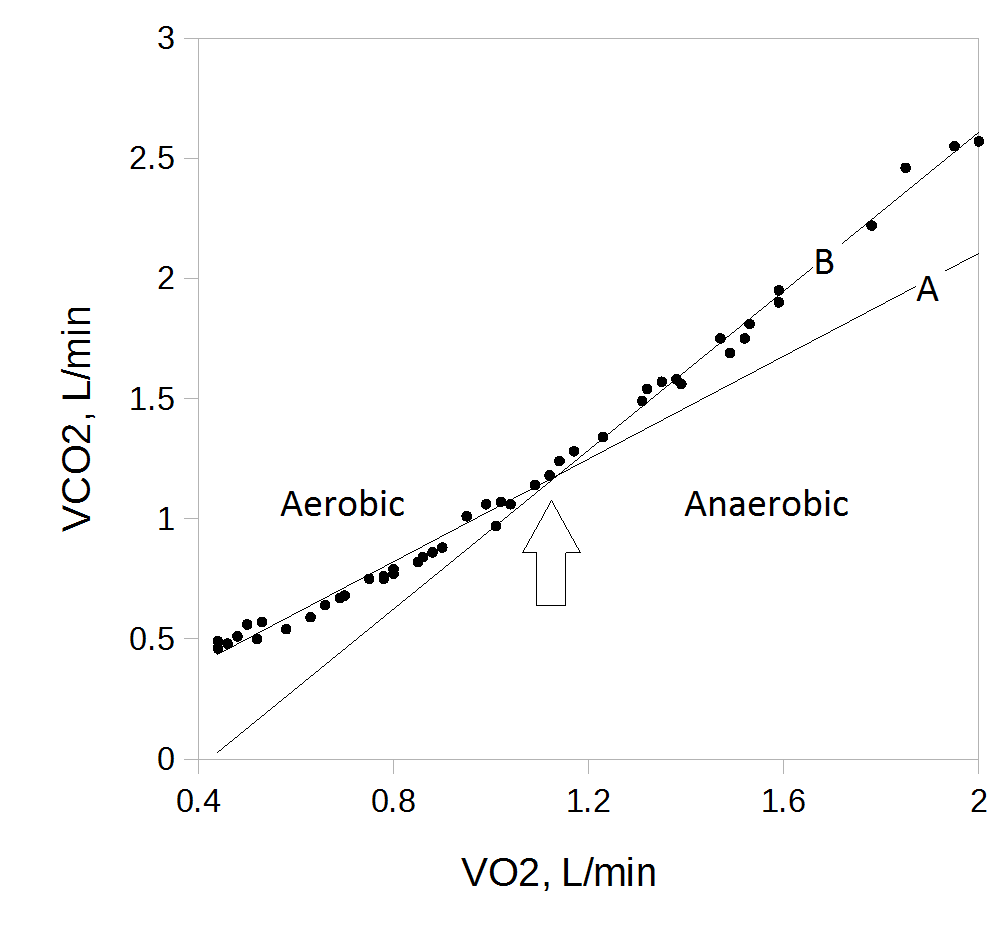
\includegraphics[width=0.7\linewidth]{../Figures/cpet_vslope}
		%\caption{Determination of $\dot{V}_{O_2}$AT by the V-slope method.}
		\label{fig:cpet_vslope}
	\end{figure}
\end{frame}

\begin{frame}
	\frametitle{Parameters measured during CPET }
	\framesubtitle{ Section 1.6 Page 25}
	\begin{itemize}
		\item
		\item
		\item
	\end{itemize}
\end{frame}

\begin{frame}
	\frametitle{Role of CPET in preoperative assessment}
	\begin{itemize}
		\item General Surgery
		\item Oesophago-gastric surgery
		\item Bariatric surgery
		\item Liver transplantation
		\item Thoracic surgery
		\medskip
		\item Little evidence in pancreatic surgery in 2010
		
	\end{itemize}
\end{frame}

\begin{frame}
	\frametitle{Aims of Thesis}
	\begin{enumerate}
		\item To evaluate the clinical utility of preoperative CPET in predicting postoperative adverse events after pancreaticoduodenectomy.
		\item To examine the patient factors that are related to cardiopulmonary exercise physiology with particular attention to the effect of obstructive jaundice and body composition.
		\item To examine the effect of preoperative systemic inflammation and poor aerobic capacity on the magnitude of the post-operative systemic inflammatory response.
		\item To examine the value of serial daily postoperative markers of systemic inflammatory response in the prediction of post-operative complications.
	\end{enumerate}
\end{frame}

\section{Methods}
\begin{frame}
	\frametitle{Patients and Methods}
	\begin{itemize}
		\item Patients undergoing pancreaticoduodenectomy at Glasgow Royal Infirmary
		\item August 2008 - August 2012
		\item Prospectively maintained MS Access database
		\item Preoperative data - Bloods, co-morbidity including POSSUM Physiology Score, stent information
		\item Cardiopulmonary exercise testing
		\item Prospective recording of complications using ISGPS or Clavie-Dindo classification
		\item Serial measurements of biochemical parameters during first postoperative week
	\end{itemize}
\end{frame}

% Discuss the results in the context of a patient.
% 63 yr old female with BMI of 35 presents with painless OJ
% PMH - HTN, T2DM, smoked 10/day for 40 yrs
% Bloods: Bil 180, CRP 22, Alb 30
% Investigations reveal an operable tumour of the head of the pancreas
% How would this patient have been managed 10 years ago?
\section{Case study}
\begin{frame}
	\frametitle{A typical patient}
	\begin{itemize}
		\item 63 yr old female with BMI of 35 presents with painless OJ
		\item PMH - HTN, T2DM, smoked 10/day for 40 yrs
		\item Bloods: Bil 180, CRP 22, Alb 30
		\item Imaging: Resectable tumour of head of pancreas
		\item How would this patient have been managed 10 years ago?
	\end{itemize}
\end{frame}

\begin{frame}
	\frametitle{10 years ago...}
	\begin{itemize}
		\item Non-dynamic measures of fitness - ECG, PFTs, ASA, ECHO
		\item Routine biliary drainage
		\item No objective methods to predict complications other than pancreatic leak
		\item Impact of postoperative SIRS on complications - no clinical utility
		\item Limited ability to identifying patients at risk of complications
		\item ERAS principles not universally applied
		\item No prehabilitation
	\end{itemize}
\end{frame}

\begin{frame}
	\frametitle{Now... }
	\begin{itemize}
		\item CPET in all or selected cases (evidence from other patient groups)
		\item Routine biliary drainage no longer indicated
		\item Enhanced recovery more widespread
		\medskip
		\hrule
		\medskip
		\item Reluctance to perform CPET in jaundiced patients
		\item No recognised thresholds for CPET parameters
		\item No clear thresholds for post-op inflammatory markers in predicting complications
		\item Poor understanding of impact of obesity on preop function and postop outcomes
		\item No prehabilitation
	\end{itemize}
\end{frame}


%--CHAPTER 2----CHAPTER 2----CHAPTER 2----CHAPTER 2----CHAPTER 2----CHAPTER 2----CHAPTER 2--
\section{Chapter 2}
\begin{frame}
	\frametitle{CPET and Postoperative Outcomes}
	\framesubtitle{Chapter 2 Page 56; (n=100)}
	\begin{block}{\textbf{Complications}}
		Low $\dot{V}_{O_2}$AT associated with pancreatic fistula (16\% vs 35\%) \\
		Not associated with cardio-respiratory complications or mortality
	\end{block}
	
	\begin{block}{\textbf{Length of stay}}
		Low $\dot{V}_{O_2}$AT associated with longer hospital stay (14 vs 20 days)\\
		Not associated with critical care stay or admissions
	\end{block}
	
	\begin{block}{\textbf{Adjuvant Therapy}}
		Low $\dot{V}_{O_2}$AT associated with non-progression to adjuvant therapy after surgery.
	\end{block}
\end{frame}

\begin{frame}
	\frametitle{CPET and Postoperative Outcomes}
	\framesubtitle{The Glasgow Cohort}
	\begin{figure}
		\centering
		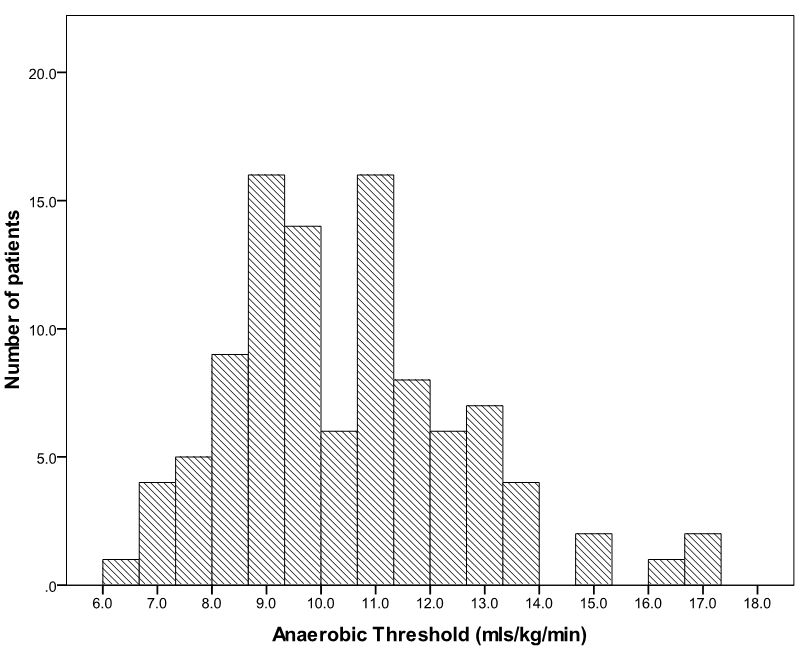
\includegraphics[height=0.35\textheight]{../Figures/cpet_outcomes_dist_of_AT}
	\end{figure}

	\begin{itemize}
		\item Median AT = 10.3 ml/kg/min (IQR 8.8 -11.6)
		\item $\dot{V}_{O_2}$AT$<$10 ml/kg/min in 49\% of patients
		\item Different from other cohorts
		\item $\dot{V}_{O_2}AT<11$ ml/kg/min in
		\begin{itemize}
			\item 16\% undergoing oesophageal surgery [Forshaw 2008]
			\item 39\% undergoing liver transplantation [Epstein 2004]
			\item 29\% undergoing abdominal surgery [Older 1993]
		\end{itemize}
	\end{itemize}
\end{frame}



\begin{frame}
	\frametitle{CPET and Postoperative Outcomes}
	\framesubtitle{Citations}
	\begin{columns}[c]
	\column{0.4\textwidth}
		\begin{figure}
			\centering
			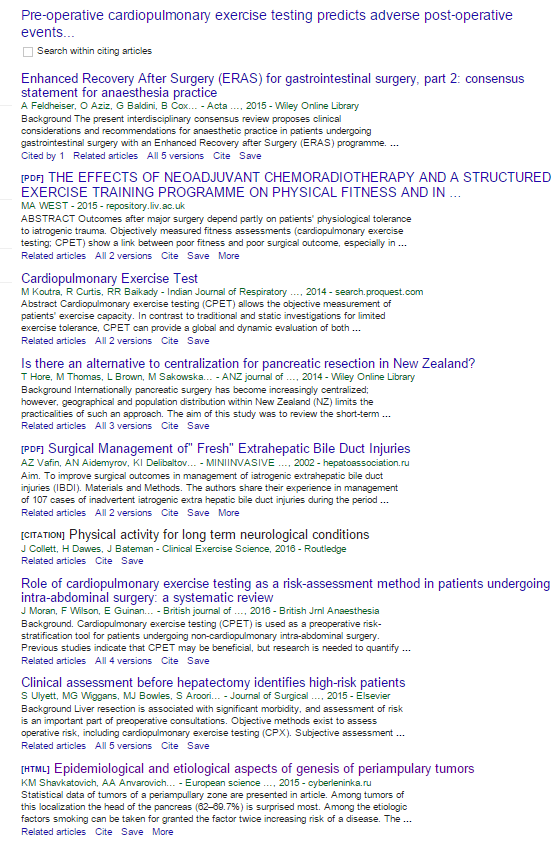
\includegraphics[width=\textwidth]{cpet_citations}
		\end{figure}
	
	\column{0.6\textwidth}
	Why is $\dot{V}_{O_2}$AT so low in patients undergoing pancreatic surgery?\\
	\medskip
	What factors are associated with a low $\dot{V}_{O_2}$AT?\\
	\medskip
	Why was $\dot{V}_{O_2}$AT not associated with cardio-respiratory complications?\\
	\medskip
	Does $\dot{V}_{O_2}$AT truely reflect cardiopulmonary function in this cohort of patients?\\	
	\end{columns}
\end{frame}


%--CHAPTER 3----CHAPTER 3----CHAPTER 3----CHAPTER 3----CHAPTER 3----CHAPTER 3----CHAPTER 3--
\section{Chapter 3}

\begin{frame}
	\frametitle{Chapter 3}
	\framesubtitle{CPET, Jaundice and Preoperative Pathophysiology - Page 76-96 }
	\begin{block}{Title}
	An investigation into the relationship between cardiopulmonary exercise testing, preoperative pathophysiology and obstructive jaundice in patients undergoing pancreaticoduodenectomy.
	\end{block}
\end{frame}

\begin{frame}
	\frametitle{Distribution of Jaundice in the study cohort }
	\framesubtitle{n=138}

	\begin{figure}
		\centering
		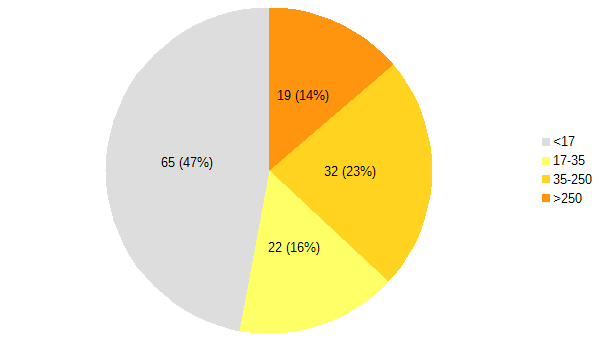
\includegraphics[width=0.7\linewidth]{jaundice_distribution}
		\caption{}
		\label{fig:jaundice_distribution}
	\end{figure}
\end{frame}



\begin{frame}
	\frametitle{Jaundice and patient characteristics}
	\framesubtitle{Table 3.1 Page 83, Table 3.2 Page 85 }
	\begin{figure}
		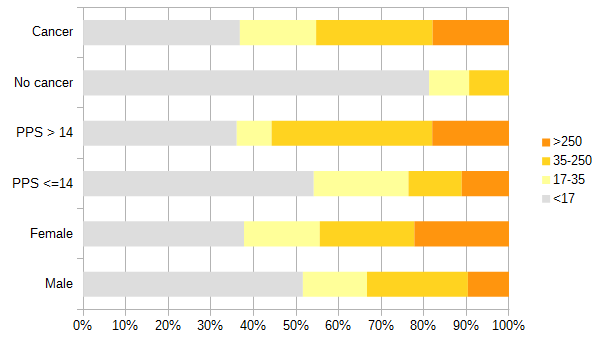
\includegraphics[height=0.4\textheight]{jaundice_vs_patient_factors}
	\end{figure}
	{\scriptsize			
	Severity of systemic inflammation proportionate to severity of jaundice. \\
	\medskip
	
	Obstructive jaundice associated with electrolyte abnormalities.\\
	\medskip			
	
	Jaundiced patients were more likely to be anaemic (p$<$0.001) with lower haematocrit (p$<$0.001) and lower mean corpuscular volume (p=0.001).\\
	\medskip
	
	No significant difference in the preoperative renal function, prothrombin time and white cell count between jaundiced and non-jaundiced patients.\\
	}
\end{frame}

\begin{frame}
	\frametitle{CPET and Jaundice}
	\framesubtitle{Figure 3.1 Page 87}
	\begin{columns}[t]
		\column{0.5\textwidth}
			\begin{figure}
				\centering
				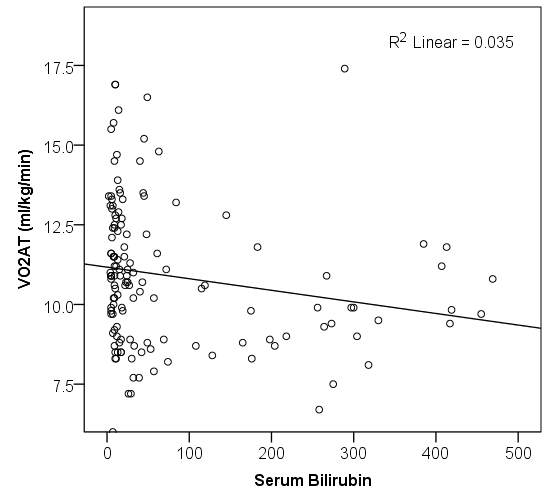
\includegraphics[width=\textwidth]{../Figures/cpet_oj_scatter_at_bil}
				\caption{$\dot{V}_{O_2}$AT versus serum bilirubin}
				\label{fig:cpet_oj_scatter_at_bil}
			\end{figure}
			
		\column{0.5\textwidth}
			\begin{figure}
				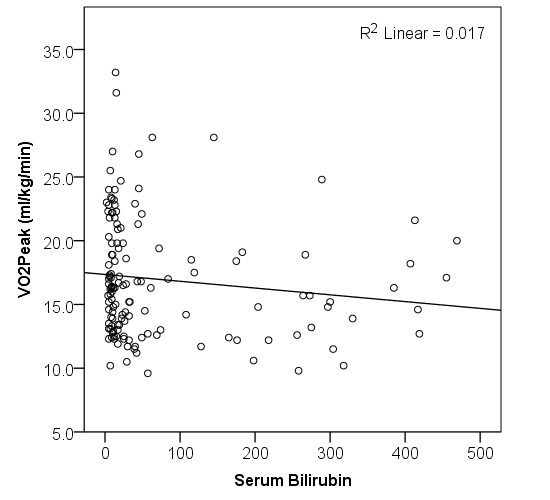
\includegraphics[width=\textwidth]{../Figures/cpet_oj_scatter_peak_bil}
				\caption{$\dot{V}_{O_2}$Peak versus serum bilirubin}
				\label{fig:cpet_oj_scatter_peak_bil}
			\end{figure}
	\end{columns}
\end{frame}


\begin{frame}
	\frametitle{$\dot{V}_{O_2}$ vs Patient Factors }
	\framesubtitle{Table 3.6 Page 91 - Multivariate binary logistic regression}

	Factors associated with $\dot{V}_{O_2}$AT $<$ 10 ml/kg/min
	\begin{table}
		\begin{tabular}{l l l l}
			           & HR   & 95\% CI    & p     \\ \hline
			Female sex & 3.75 & 1.57-8.95  & 0.003 \\
			BMI$>$25   & 3.65 & 1.61-8.26  & 0.002 \\
			Cancer     & 4.02 & 1.33-12.16 & 0.014 \\
			CRP$>$10   & 2.98 & 1.29-6.86  & 0.010
		\end{tabular}
	\end{table}
	
	Factors associated with $\dot{V}_{O_2}$Peak $<$ 16ml/kg/min
	\begin{table}
		\begin{tabular}{l l l l}
			            & HR   & 95\% CI   & p        \\ \hline
			Female sex  & 7.57 & 3.09-18.5 & $<$0.001 \\
			BMI$>$25    & 2.57 & 1.18-5.63 & 0.018    \\
			Haemoglobin & 2.43 & 1.05-5.63 & 0.038
		\end{tabular}
	\end{table}
\end{frame}


%--CHAPTER 4----CHAPTER 4----CHAPTER 4----CHAPTER 4----CHAPTER 4----CHAPTER 4----CHAPTER 4--
\section{Chapter 4}

\begin{frame}
	\frametitle{Chapter 4}
	\framesubtitle{CPET and Body Composition - Page 97-122 }
	\begin{block}{Title}
		An investigation into the relationship between cardiopulmonary exercise testing and body composition in patients undergoing pancreaticoduodenectomy.
	\end{block}
\end{frame}

\begin{frame}
	\frametitle{What causes a low $\dot{V}_{O_2}$? }
	\framesubtitle{Section 4.1.2 Page 98-99 }
	\begin{itemize}
		\item Low $\dot{V}_{O_2}$ has been universally ascribed to low aerobic fitness due to inadequate cardio-pulmonary reserve
		\item Occassionally anaemia, peripheral vascular disease or even mitochondrial diseases may play a role
		\item $\dot{V}_{O_2}$AT and $\dot{V}_{O_2}$Peak are most commonly used parameters
		\item Both are normalised by dividing using patient's total body weight
		\item But, during exercise $\dot{V}_{O_2}$ is a function of skeletal muscle mass
		\item This can result in 'spurious correlation' unfairly penalising obese subjects
		\item Most patients in this cohort did not have overt cardiac/respiratory disease that could explain the low $\dot{V}_{O_2}$.
	\end{itemize}
\end{frame}

\begin{frame}
	\frametitle{Corrected $\dot{V}_{O_2}$ vs. Absolute $\dot{V}_{O_2}$}
	\framesubtitle{Could this be a source of spurious correlation?}
	
	\[Corrected\ \dot{V}_{O_2} (ml/kg/min) = \frac{Absolute\ \dot{V}_{O_2}\ (litres/min) * 1000}{Total\ body\ weight\ (kg)}\]

	\vfill
	
	For example, if the absolute $\dot{V}_{O_2}$AT was 0.84 litres/min, the corrected $\dot{V}_{O_2}$AT (ml/kg/min) would vary with patient weight as follows:
	
	\begin{table}
	\begin{tabular}{c c c c c c}
		     Weight       & kg        & 70 & 80   & 90  & 100 \\
		$\dot{V}_{O_2}$AT & ml/kg/min & 12 & 10.5 & 9.3 & 8.4
	\end{tabular}
	\end{table}


\end{frame}

\begin{frame}
	\frametitle{Body composition estimation}
	\framesubtitle{Figure 4.1 Page 103}
	\begin{figure}
		\centering
		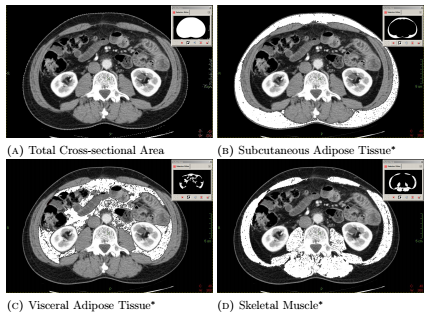
\includegraphics[width=\linewidth]{bc_gimp}
		\label{fig:bc_gimp}
	\end{figure}
\end{frame}

\begin{frame}
	\frametitle{$\dot{V}_{O_2}$AT vs Skeletal Muscle}
	\framesubtitle{Figure 4.4(A) Page 111, Figure 4.5(A) on Page 114}


	\begin{figure}
		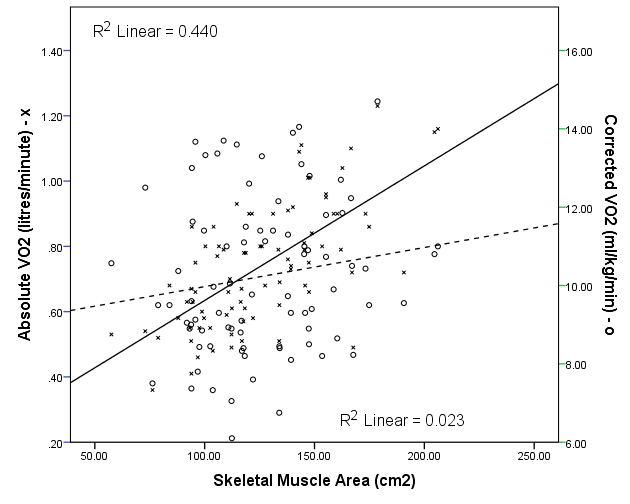
\includegraphics[height=0.4\textheight]{../Figures/bc_scatter_VO2_skeletal}
	\end{figure}

	\begin{figure}
		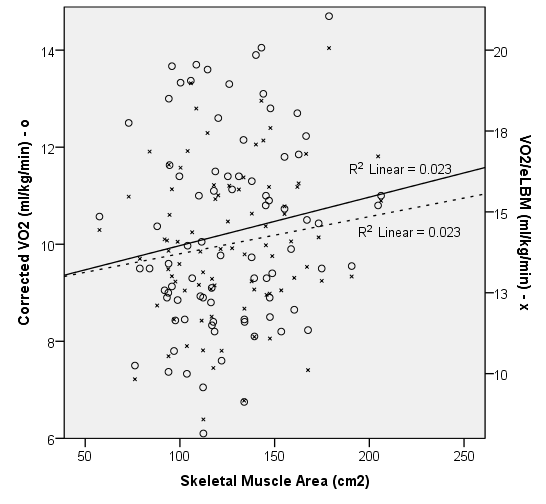
\includegraphics[height=0.45\textheight]{../Figures/bc_scatter_VO2_skeletal_elbm}
	\end{figure}
	
\end{frame}

\begin{frame}
	\frametitle{$\dot{V}_{O_2}$AT vs Total Adipose Tissue}
	\framesubtitle{Figure 4.4(B) Page 111, Figure 4.5(B) on Page 114}

	\begin{figure}
		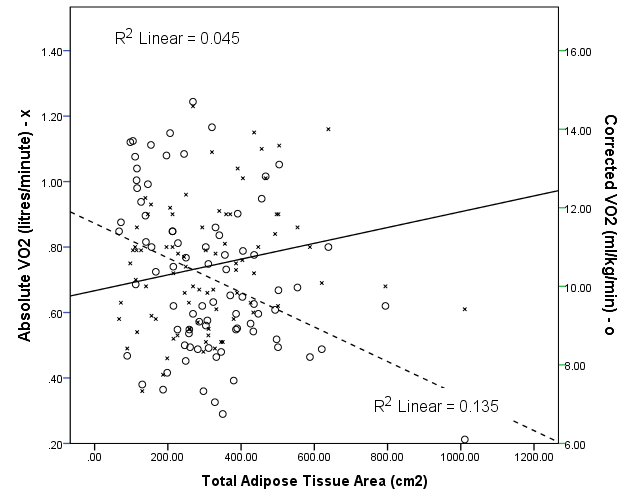
\includegraphics[height=0.4\textheight]{../Figures/bc_scatter_VO2_TAT}
	\end{figure}
	\begin{figure}
		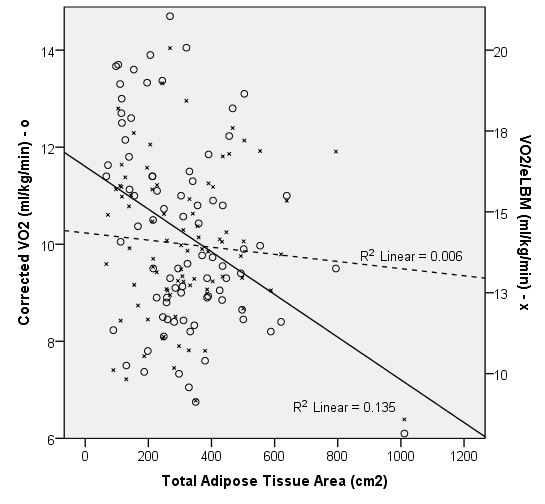
\includegraphics[height=0.45\textheight]{../Figures/bc_scatter_VO2_TAT_elbm}
	\end{figure}
	
\end{frame}



\section{Chapter 5}

\begin{frame}
	\frametitle{Chapter 5}
	\begin{block}{Title}
		An investigation into the relationship between preoperative clinico-pathological characteristics and post-operative systemic inflammatory response in patients undergoing pancreaticoduodenectomy.
	\end{block}
\end{frame}

\begin{frame}
	\frametitle{Background}
	\framesubtitle{Section 5.1 Page 124}
	\begin{itemize}
		\item Perioperative systemic inflammation influences short and long-term outcomes
		\item Elevated preoperative systemic inflammation is associated with postoperative complications in colorectal surgery, after oesophagectomy, liver resections and cardiac surgery. 
		\item Early exaggerated postoperative systemic inflammatory response is also associated with increased infective complications
		\item In patients undergoing pancreatic surgery, preoperative inflammatory state is further influenced by:
		\begin{itemize}
			\item Obstructive jaundice
			\item Cholangitis
			\item ERCP and stenting
			\item Post-ERCP / EUS related complications
		\end{itemize}
		\item Obesity is associated with chronic inflammation
		\item Impact of aerobic capacity on postoperative inflammation not studied before
	\end{itemize}
\end{frame}


\begin{frame}
	\frametitle{Preop inflammation vs. Postop CRP}
	\framesubtitle{Figure 5.3 Page 142}
	\begin{figure}
		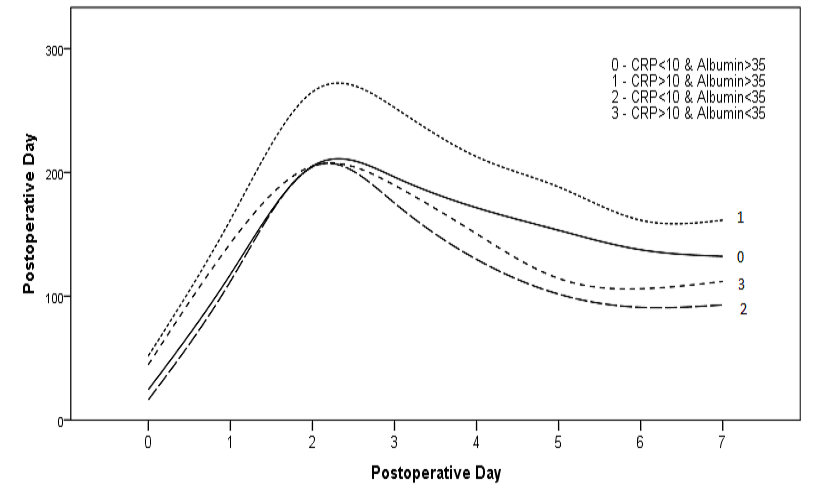
\includegraphics[width=\textwidth]{../Figures/sirs_crp_crp_alb}
	\end{figure}
\end{frame}

\begin{frame}
	\frametitle{Obstructive jaundice vs. Postop CRP}
	\framesubtitle{ }
	\begin{figure}
		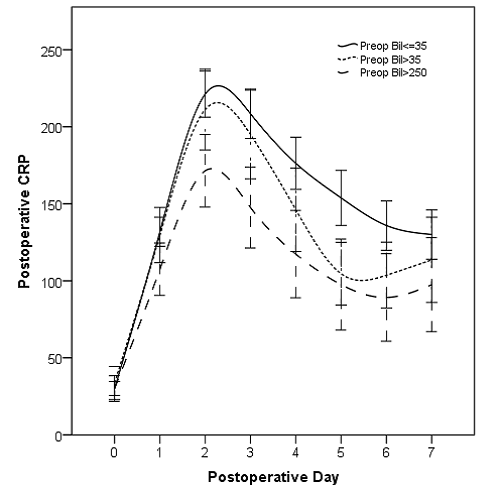
\includegraphics[width=0.7\textwidth]{../Figures/sirs_bil_crp}
	\end{figure}

\end{frame}

\begin{frame}
	\frametitle{CPET, Body composition vs. Postop Inflammation }
	\framesubtitle{Section 5.3.4, 5.3.5 Pages 132-133, Tables 5.8-5.10 Pages 145-147 }
	\begin{itemize}
		\item No relationship between $\dot{V}_{O_2}$ and post op. CRP or neutrophil count
		\vfill
		\item Serum albumin levels lower in patients with low VO2
		\begin{itemize}
			\item Probably related to preop hypoalbuminemia
			\item This in turn related to low skeletal muscle and multiple other factors
		\end{itemize}
		\vfill
		\item No relationship between body composition and postoperative CRP/neutrophil counts
	\end{itemize}
\end{frame}


\section{Chapter 6}
\begin{frame}
	\frametitle{Chapter 6}
	\framesubtitle{Postoperative CRP and complications}
	\begin{block}{Title}
		An investigation into the relationship between postoperative systemic inflammation and complications after pancreaticoduodenectomy.
	\end{block}
\end{frame}

\begin{frame}
	\frametitle{Does post op. CRP predict severity of POPF?}
	\framesubtitle{No, it does not. \\ Moreover, diagnosis of POPF is made on the third day using drain amylase. }
	
	\begin{columns}
		\column[c]{0.45\textwidth}
			\begin{figure}
				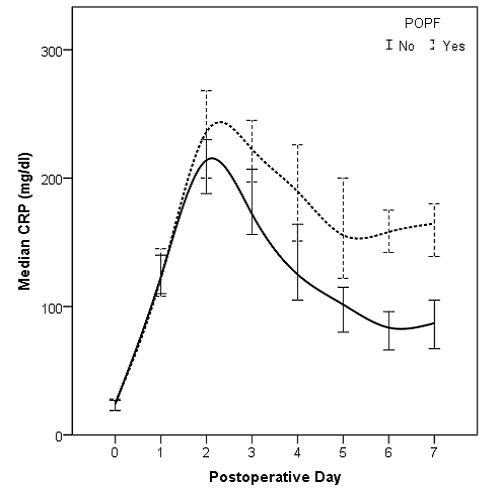
\includegraphics[width=\textwidth]{../Figures/crp_comp_crp_popf_yes_no}
			\end{figure}
		
		\column[c]{0.45\textwidth}
			\begin{figure}
				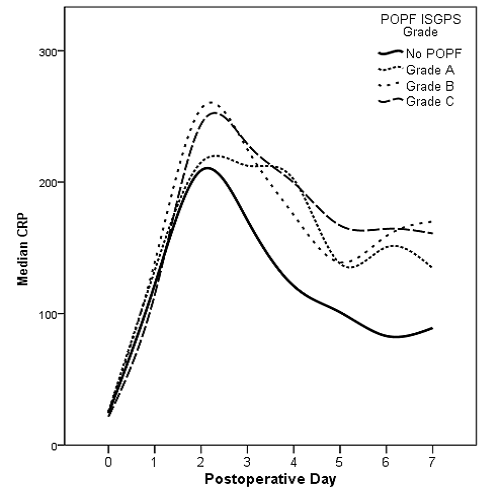
\includegraphics[width=\textwidth]{../Figures/crp_comp_crp_popf_isgps}
			\end{figure}
	\end{columns}

\end{frame}

\begin{frame}
	\frametitle{Does post op. CRP predict infective complications?}
	\framesubtitle{Yes, it does. \\ But, only in the absence of a pancreatic fistula. }
	
	\begin{columns}
		\column[c]{0.45\textwidth}
		\begin{figure}
			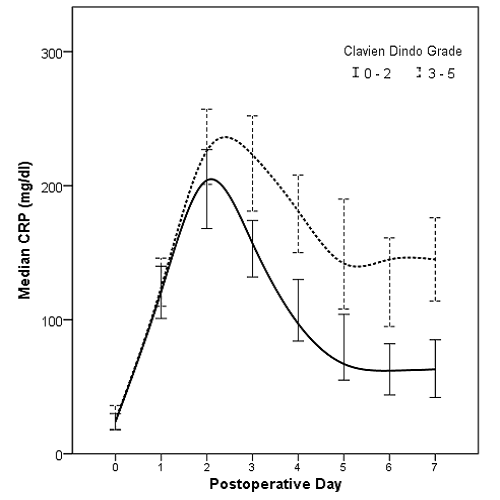
\includegraphics[width=\textwidth]{../Figures/crp_comp_infective_leak0}
			\\ Patients with NO POPF
		\end{figure}
		
		\column[c]{0.45\textwidth}
		\begin{figure}
			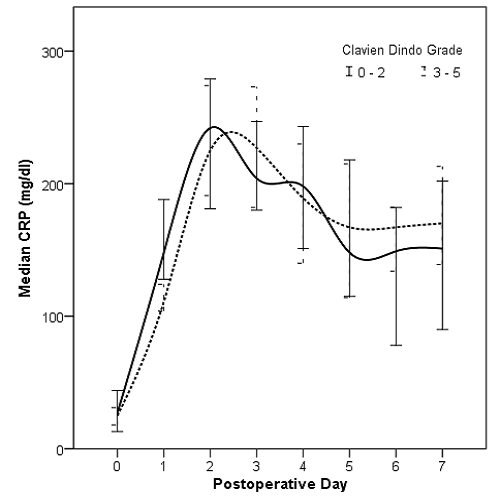
\includegraphics[width=\textwidth]{../Figures/crp_comp_infective_leak1}
			\\ Patients with POPF
		\end{figure}
	\end{columns}
\end{frame}

\begin{frame}
	\frametitle{Receiver operating characteristics analysis}
	\framesubtitle{CRP thresholds for predicting infective complications in the absence of a POPF. }
	\begin{columns}
		\column[c]{0.45\textwidth}
			\begin{figure}
				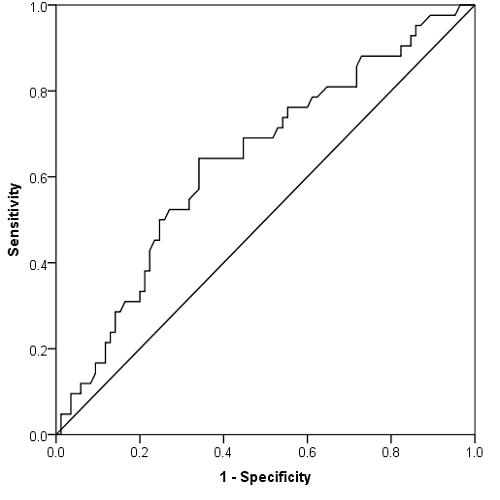
\includegraphics[width=\textwidth]{../Figures/crp_comp_ROC_infection_D3}
				\\{\scriptsize D3 178 mg/dl; AUC 0.64; NPV 0.79; \\Spec 0.66; Sens 0.64; p=0.011}
			\end{figure}
		\column[c]{0.45\textwidth}
			\begin{figure}
				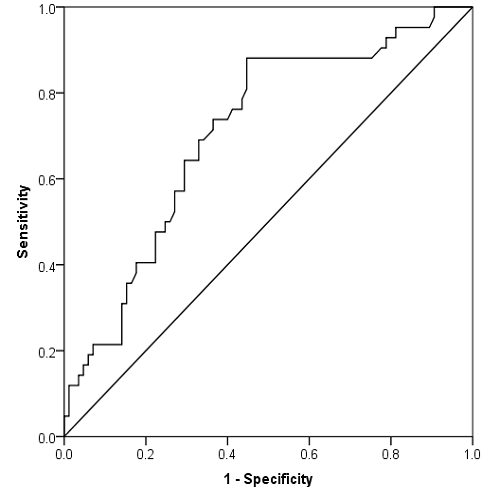
\includegraphics[width=\textwidth]{../Figures/crp_comp_ROC_infection_D4}
				\\{\scriptsize D4 125 mg/dl; AUC 0.71; NPV 0.83; \\Spec 0.64; Sens 0.74; p$<$0.001}
			\end{figure}
	\end{columns}
\end{frame}







%------------------------------------------------

\begin{frame}[fragile] % Need to use the fragile option when verbatim is used in the slide
\frametitle{Verbatim}
\begin{example}[Theorem Slide Code]
\begin{verbatim}
\begin{frame}
\frametitle{Theorem}
\begin{theorem}[Mass--energy equivalence]
$E = mc^2$
\end{theorem}
\end{frame}\end{verbatim}
\end{example}
\end{frame}


%------------------------------------------------

\begin{frame}
\Huge{\centerline{The End}}
\end{frame}

%----------------------------------------------------------------------------------------

\end{document} 